\documentclass[
  article,
  12pt,
  oneside,
  a4paper,
  english,
  brazil,
  chapter=TITLE,
  section=TITLE,
  subsection=TITLE
]{abntex2}

\usepackage[T1]{fontenc}
\usepackage[utf8]{inputenc}
\usepackage{newtxtext,newtxmath}
\usepackage{indentfirst}
\usepackage{graphicx}
\usepackage{microtype}
\usepackage{placeins}
\usepackage{listingsutf8}

\lstset{
  inputencoding=utf8/latin1,
  language=Python,
  basicstyle=\ttfamily\footnotesize,
  breaklines=true,
  columns=fullflexible,
  keepspaces=true,
  showstringspaces=false,
  tabsize=2,
  frame=single,
  numbers=left,
  numberstyle=\tiny,
  numbersep=8pt,
  xleftmargin=2em,
  framexleftmargin=1.6em,
  aboveskip=8pt,
  belowskip=8pt
}

\makeatletter
\g@addto@macro{\UrlBreaks}{\do\_}
\makeatother

\titulo{Classificação do impacto das redes sociais com MLP e SVM}
\autor{Ian de Araújo \and Jardson Alan}
\local{Rio Grande do Norte}
\data{2026}
\instituicao{%
  Instituto Federal de Educação, Ciência e Tecnologia\\
  do Rio Grande do Norte%
}
\preambulo{%
  Artigo apresentado à disciplina de Análise de Dados do Instituto Federal
  de Educação, Ciência e Tecnologia do Rio Grande do Norte, com o registro
  da etapa de classificação com rede neural MLP e máquina de vetores de suporte (SVM).%
}

\hypersetup{
  hidelinks,
  pdftitle={Classificação do impacto das redes sociais com MLP e SVM},
  pdfauthor={Ian de Araújo; Jardson Alan}
}

\renewcommand{\imprimircapa}{%
  \begin{capa}%
    \SingleSpacing
    \begin{center}
      \imprimirinstituicao\par
      \vspace*{\fill}
      \imprimirautor\par
      \vspace*{\fill}
      {\bfseries\imprimirtitulo\par}
      \vspace*{\fill}
      \imprimirlocal\par
      \imprimirdata\par
    \end{center}
    \vspace*{1cm}
  \end{capa}%
}

\renewcommand{\folhaderostocontent}{%
  \SingleSpacing
  \begin{center}
    \imprimirautor\par
  \end{center}
  \vspace{3.2cm}
  \begin{center}
    {\bfseries\imprimirtitulo\par}
  \end{center}
  \vspace{2.2cm}
  \hfill
  \begin{minipage}[t]{.46\textwidth}
    \imprimirpreambulo
  \end{minipage}
  \vspace{3.2cm}
  \begin{center}
    \imprimirlocal\par
    \imprimirdata\par
  \end{center}
}

\AtBeginDocument{%
  \setlength{\absleftindent}{0pt}%
  \setlength{\absrightindent}{0pt}%
  \setlength{\absparindent}{0pt}%
  \setlength{\emergencystretch}{2.5em}%
}

\graphicspath{{../figures/}}

\begin{document}

\pretextual
\imprimircapa
\imprimirfolhaderosto

\textual

\begin{center}
  \bfseries\imprimirtitulo
\end{center}

\vspace{0.75\baselineskip}
\noindent Ian de Araújo\footnotemark{} e Jardson Alan\footnotemark[\value{footnote}]
\footnotetext{Estudantes da disciplina de Análise de Dados do Instituto Federal de Educação, Ciência e Tecnologia do Rio Grande do Norte.}

\begin{resumo}
Esta etapa classifica o impacto das redes sociais em 4.500 estudantes com uma rede neural \emph{multilayer perceptron} (MLP) e com uma máquina de vetores de suporte (SVM). A classe é \texttt{Overall\_Impact}, com os rótulos \texttt{Beneficial}, \texttt{Neutral} e \texttt{Negative}. As entradas são as sete medidas numéricas do agrupamento, padronizadas dentro de um \texttt{Pipeline}, e o índice de saúde mental fica de fora. Os hiperparâmetros dos dois modelos são escolhidos por \texttt{GridSearchCV} no recorte de treino. A MLP escolhida tem duas camadas ocultas (64 e 32 neurônios) e ativação ReLU. O SVM escolhido usa kernel linear e $C = 1$. Pela validação cruzada de cinco partes, feita por \texttt{cross\_val\_score}, a acurácia média é 0,9596 na MLP e 0,9633 no SVM. Os dois ficam acima do Naive Bayes, da árvore de decisão e do k-NN.

\vspace{\onelineskip}
\noindent
\textbf{Palavras-chave}: Classificação. Redes neurais. SVM. Validação cruzada. Redes sociais.
\end{resumo}

\section{Etapa de classificação com MLP e SVM}

O objetivo é prever a classe já existente em \texttt{Overall\_Impact}, como nos outros classificadores. Há 3.681 registros \texttt{Beneficial}, 654 \texttt{Neutral} e 165 \texttt{Negative}. O arquivo é \texttt{data/raw/}\allowbreak\texttt{dataset.csv}, com 4.500 estudantes (YADAV, 2026).

A rede MLP combina entradas ponderadas em camadas de neurônios com função de ativação não linear, e aprende os pesos por retropropagação do erro. O SVM procura a fronteira que separa as classes com a maior margem, e o kernel permite fronteiras não lineares. Os dois são sensíveis à escala dos atributos. Por isso a padronização com \texttt{StandardScaler} fica dentro de um \texttt{Pipeline}, antes do modelo, e é aprendida só nos dados de treino de cada parte da busca e da validação cruzada. Isso evita que informação do teste vaze para o treino.

As entradas vêm de \texttt{prepare\_data}, em \texttt{src/clustering/}\allowbreak\texttt{grouping.py}, que preenche os vazios de estresse e de GPA com a média truncada por idade. Aqui é usada a primeira saída da função, sem padronizar. São sete colunas numéricas: idade, horas diárias, horas extras de fim de semana, duração e qualidade do sono, estresse percebido e GPA. \texttt{Student\_ID} e \texttt{Mental\_Health\_Index} não entram, e a classe também não.

O recorte é o mesmo dos outros classificadores, com 33\% dos registros para teste e semente 125. A comparação feita pela etapa é a validação cruzada de cinco partes, com acurácia, aplicada por \texttt{cross\_val\_score}.

\section{Rede neural MLP}

O \texttt{MLPClassifier} usa o otimizador \texttt{adam}, no máximo 500 iterações e parada antecipada: 20\% do treino ficam como validação interna, e o treino termina depois de 20 iterações sem melhora. O \texttt{GridSearchCV} testa 48 combinações, com cinco partes internas e acurácia como critério:

\begin{itemize}
  \item camadas ocultas: (32), (32, 16), (64, 32) e (64, 32, 16);
  \item ativação: \texttt{relu} ou \texttt{tanh};
  \item regularização \texttt{alpha}: 0,0001, 0,001 ou 0,01;
  \item taxa de aprendizado inicial: 0,001 ou 0,01.
\end{itemize}

O conjunto escolhido foi duas camadas ocultas de 64 e 32 neurônios, ativação \texttt{relu}, \texttt{alpha} de 0,0001 e taxa de 0,01, com acurácia média de 0,9632 na busca. A rede parou em 27 iterações, como na Figura~\ref{fig:mlp}. Uma rede nova, com esses hiperparâmetros, foi avaliada por \texttt{cross\_val\_score} no conjunto inteiro. A média foi 0,9596 e o desvio-padrão 0,0057, como na Tabela~\ref{tab:cv}. A taxa de aprendizado escolhida é o maior valor da grade.

\begin{figure}[htb]
  \centering
  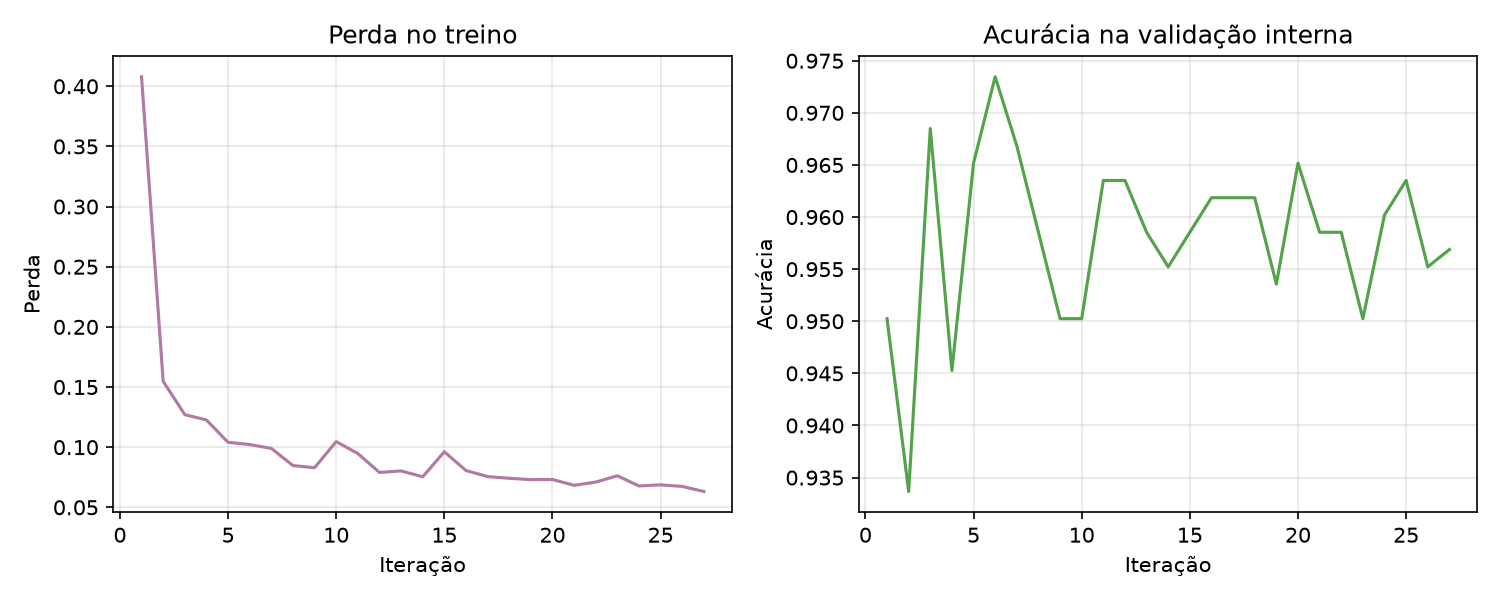
\includegraphics[width=\textwidth]{mlp_training.png}
  \caption{Treino da MLP escolhida: perda e acurácia na validação interna}
  \label{fig:mlp}
  \fonte{Elaborado pelos autores (2026), pela execução do classificador.}
\end{figure}

No recorte de teste, a acurácia da MLP foi 0,9401, a acurácia balanceada 0,8735 e a área sob a curva ROC, em média macro um contra os demais, 0,9912. A Tabela~\ref{tab:mlp} mostra a matriz. A MLP é o modelo que mais recupera os \texttt{Neutral} (205 de 229), mas troca 53 \texttt{Beneficial} por \texttt{Neutral}.

\begin{table}[htb]
  \centering
  \caption{Matriz da MLP no recorte de teste}
  \label{tab:mlp}
  \begin{tabular}{lrrr}
    \toprule
    Real & Beneficial & Negative & Neutral \\
    \midrule
    Beneficial & 1151 & 0 & 53 \\
    Negative & 0 & 40 & 12 \\
    Neutral & 18 & 6 & 205 \\
    \bottomrule
  \end{tabular}
  \fonte{Elaborado pelos autores (2026), pela execução do classificador.}
\end{table}

\section{SVM}

O \texttt{SVC} também passa por \texttt{GridSearchCV}, com cinco partes internas e acurácia como critério. A grade tem 40 combinações. O kernel linear é testado com \texttt{C} igual a 0,1, 1, 10 ou 100 e com \texttt{class\_weight} \texttt{None} ou \texttt{balanced}. O kernel \texttt{rbf} é testado com os mesmos valores de \texttt{C} e \texttt{class\_weight}, e com \texttt{gamma} igual a \texttt{scale}, 0,01, 0,1 ou 1. O \texttt{gamma} só tem efeito no \texttt{rbf}, por isso o kernel linear tem uma grade própria.

O conjunto escolhido foi kernel linear, $C = 1$ e sem pesos de classe, com acurácia média de 0,9645 na busca. A média da validação cruzada, com um SVM novo e esses hiperparâmetros, foi 0,9633 e o desvio-padrão 0,0017, o menor entre os cinco classificadores. O kernel linear vencer o \texttt{rbf} indica que as classes são bem separadas por fronteiras lineares nessas sete variáveis.

\begin{table}[htb]
  \centering
  \caption{Acurácia na validação cruzada de cinco partes}
  \label{tab:cv}
  \small
  \begin{tabular}{lrrrrrr}
    \toprule
    Modelo & Parte 1 & Parte 2 & Parte 3 & Parte 4 & Parte 5 & Média \\
    \midrule
    Naive Bayes & 0,9278 & 0,9289 & 0,9233 & 0,9067 & 0,9322 & 0,9238 \\
    Árvore de decisão & 0,9544 & 0,9444 & 0,9556 & 0,9356 & 0,9500 & 0,9480 \\
    k-NN (k = 3) & 0,9522 & 0,9378 & 0,9511 & 0,9444 & 0,9367 & 0,9444 \\
    MLP & 0,9656 & 0,9600 & 0,9600 & 0,9489 & 0,9633 & 0,9596 \\
    SVM (linear) & 0,9667 & 0,9622 & 0,9622 & 0,9622 & 0,9633 & 0,9633 \\
    \bottomrule
  \end{tabular}
  \fonte{Elaborado pelos autores (2026), pela execução dos classificadores.}
\end{table}

No recorte de teste, a acurácia do SVM foi 0,9596, a acurácia balanceada 0,8893 e a área sob a curva ROC 0,9896. Esta última usa a distância à fronteira de decisão, e não probabilidades como na MLP. A Tabela~\ref{tab:svm} e a Figura~\ref{fig:matrizes} mostram as matrizes. O SVM acerta 1.186 dos 1.204 \texttt{Beneficial}, 43 dos 52 \texttt{Negative} e 196 dos 229 \texttt{Neutral}.

\begin{table}[htb]
  \centering
  \caption{Matriz do SVM no recorte de teste}
  \label{tab:svm}
  \begin{tabular}{lrrr}
    \toprule
    Real & Beneficial & Negative & Neutral \\
    \midrule
    Beneficial & 1186 & 0 & 18 \\
    Negative & 0 & 43 & 9 \\
    Neutral & 28 & 5 & 196 \\
    \bottomrule
  \end{tabular}
  \fonte{Elaborado pelos autores (2026), pela execução do classificador.}
\end{table}

\begin{figure}[htb]
  \centering
  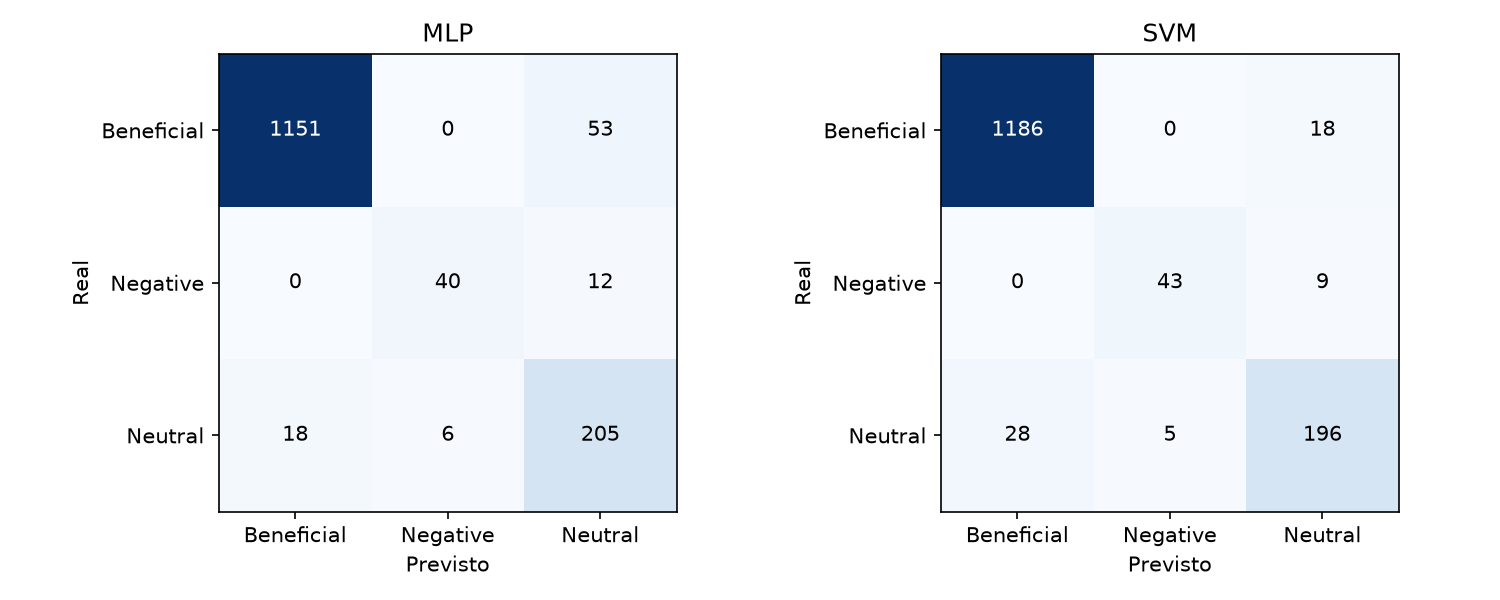
\includegraphics[width=\textwidth]{mlp_svm_confusion_matrices.png}
  \caption{Matrizes de confusão da MLP e do SVM no recorte de teste}
  \label{fig:matrizes}
  \fonte{Elaborado pelos autores (2026), pela execução dos classificadores.}
\end{figure}

\section{Comparativo}

Pela média da validação cruzada, o SVM (0,9633) fica à frente da MLP (0,9596), e os dois ficam acima da árvore de decisão (0,9480), do k-NN (0,9444) e do Naive Bayes (0,9238), como na Figura~\ref{fig:comparativo}. A diferença entre SVM e MLP, de 0,0037, é menor que o desvio-padrão das partes da MLP, então não separa os dois com segurança. O SVM é também o mais estável, com desvio de 0,0017. No recorte de teste, o SVM tem a maior acurácia (0,9596), seguido pela árvore (0,9434), por k-NN e MLP (0,9401) e pelo Naive Bayes (0,9178). Na MLP, a acurácia no teste ficou abaixo da média da validação cruzada.

\begin{figure}[htb]
  \centering
  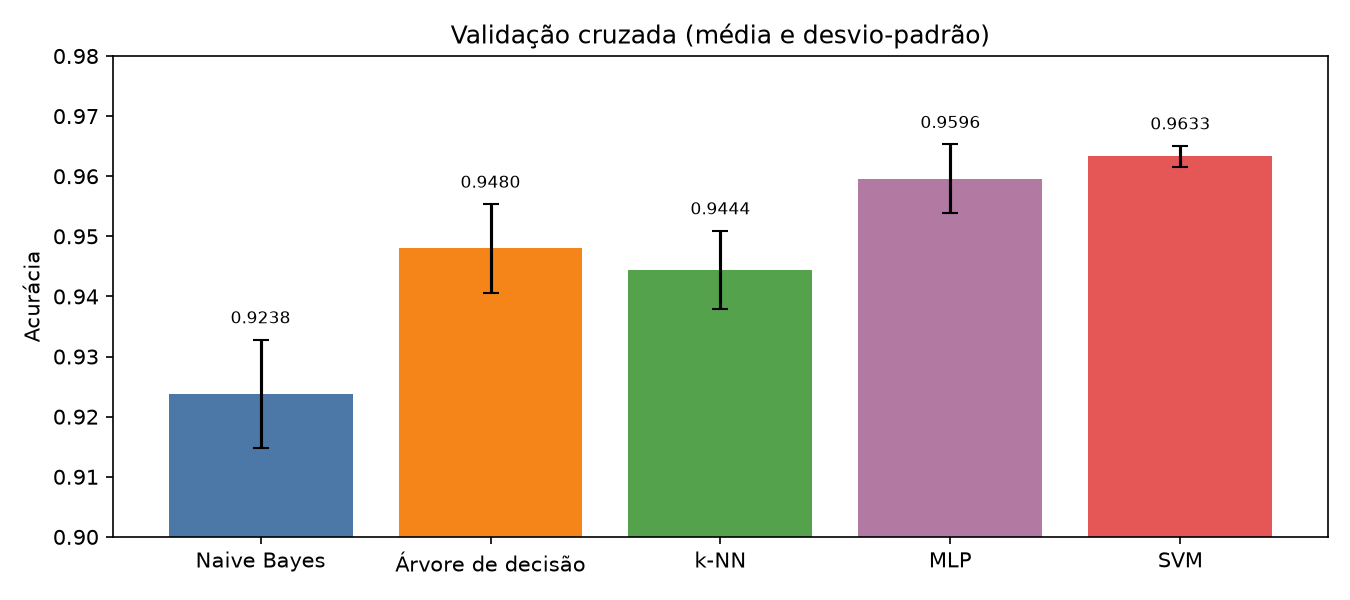
\includegraphics[width=0.9\textwidth]{models_cross_validation.png}
  \caption{Acurácia média e desvio-padrão da validação cruzada dos cinco classificadores}
  \label{fig:comparativo}
  \fonte{Elaborado pelos autores (2026), pela execução dos classificadores.}
\end{figure}

A classe \texttt{Beneficial} é a maioria do arquivo (81,8\%), então a acurácia dos cinco já parte de um patamar alto. Nas classes pequenas, o Naive Bayes acerta mais \texttt{Negative} (49 de 52), contra 44 da árvore, 43 do SVM, 40 da MLP e 38 do k-NN. Nos \texttt{Neutral}, a MLP acerta mais (205 de 229), seguida pelo SVM (196) e pelo Naive Bayes (194).

\FloatBarrier

\section{Código utilizado}

As listagens são os arquivos desta etapa, como estão no repositório. \texttt{main.py} chama os classificadores e a função que grava as figuras. \texttt{mlp.py} escolhe os hiperparâmetros da rede com \texttt{GridSearchCV} e avalia a rede escolhida com \texttt{cross\_val\_score}. \texttt{svm.py} faz o mesmo para o SVM. \texttt{charts.py} grava os gráficos em \texttt{reports/figures/}.

\subsection{Chamada no fluxo}

Arquivo \texttt{main.py}.

\lstinputlisting{../../../main.py}

\subsection{Rede neural MLP}

Arquivo \texttt{src/classifiers/}\allowbreak\texttt{mlp.py}.

\lstinputlisting{../../../src/classifiers/mlp.py}

\subsection{SVM}

Arquivo \texttt{src/classifiers/}\allowbreak\texttt{svm.py}.

\lstinputlisting{../../../src/classifiers/svm.py}

\subsection{Gráficos}

Arquivo \texttt{src/visualization/}\allowbreak\texttt{charts.py}.

\lstinputlisting{../../../src/visualization/charts.py}

\postextual

\begin{thebibliography}{9}
\bibitem{yadav2026}
YADAV, Harish. \textbf{Impact of Social Media on Life}. 2026. Conjunto de dados. Disponível em: \url{https://www.kaggle.com/datasets/harishyadav0506/impact-of-social-media-on-life}. Acesso em: 9 nov. 2026.
\end{thebibliography}

\end{document}
